\section{Classifiers Implementation}

Following the selection of the dataset, the \gls{DNA} sequence records were randomly rearranged and assigned to the training and test/validation sets. A suitable data preprocessing strategy was selected in order to turn the \gls{DNA} sequences, into a numerical representation. This format was necessary to comply with the input requirements of the classification model, which takes only numerical data.

At this stage, there will be either a collection of pre-calculated features, the descriptors, or labeled and encoded training data. The data will be used to train the classification model regardless of the previous choice.

\subsection{Models}

The following sections will provide an insight for each one of the implemented classification models.

\begin{figure}[htbp]
    \centering
    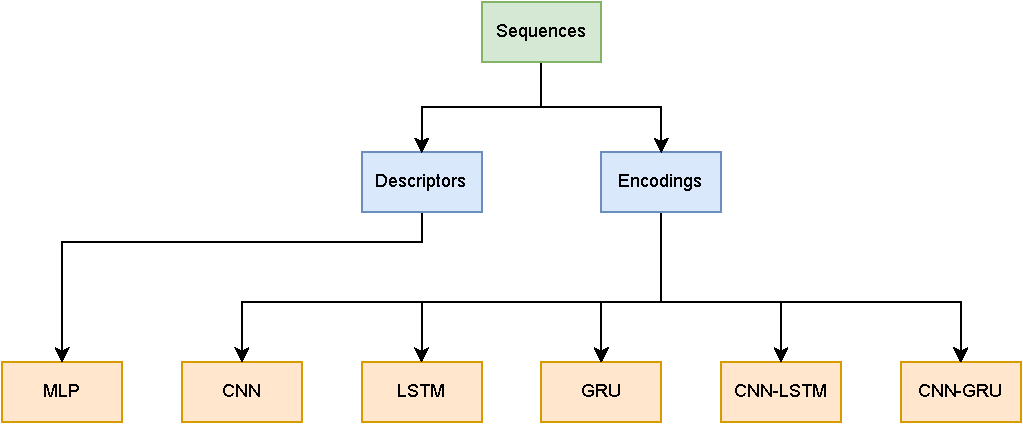
\includegraphics[width=0.7\linewidth]{models_feature_extraction}
    \caption{Models and their feature extraction methods.}
    \label{fig:models_feature_extraction}
\end{figure}

\paragraph{MLP}

The first model is a feedforward artificial neural network called \gls{MLP}. This is the only model that can take the descriptors as input data, since it is only the shallow \gls{ML} model implemented. Figure~\ref{fig:mlp-arch} shows its architecture, which was based in a~\citeauthor{Zhang2020DeepHE:Learning}'s research~\cite{Zhang2020DeepHE:Learning}, one of the cases studies of this thesis.

\begin{figure}[htbp]
    \centering
    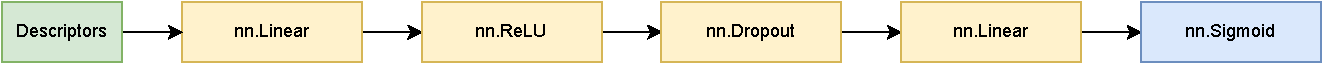
\includegraphics[width=0.8\linewidth]{mlp-arch}
    \caption{MLP architecture.}
    \label{fig:mlp-arch}
\end{figure}

\paragraph{CNN}

The \gls{CNN} model, which was also inspired by one of this thesis' case studies, specifically~\citeauthor{Zou2018AGenomics}'s research~\cite{Zou2018AGenomics} and is depicted in Figure~\ref{fig:cnn-arch}. 

\begin{figure}[htbp]
    \centering
    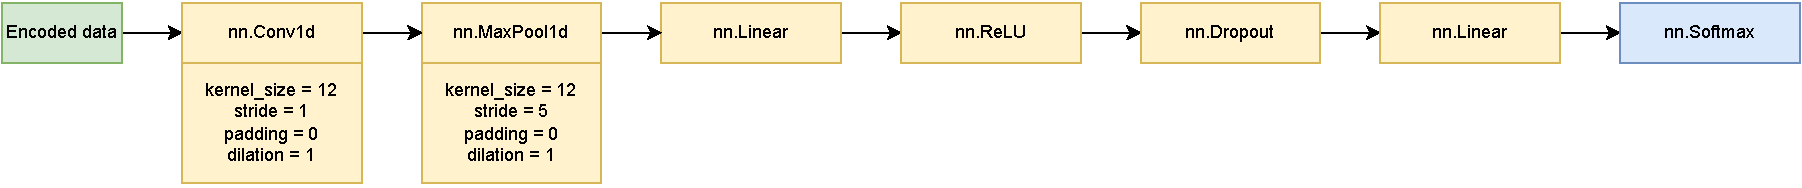
\includegraphics[width=\linewidth]{cnn-arch}
    \caption{CNN architecture.}
    \label{fig:cnn-arch}
\end{figure}

\paragraph{LSTM / BiLSTM}

This \gls{LSTM} model is a simple model regarding the number of layers, but it is possible to pass to the \textit{nn.LSTM} layer a parameter called $num\_layers$ that specifies the number of recurrent layers. Setting $num \_layers = 2$ would result in a stacked \gls{LSTM}, which would consist of two \gls{LSTM}s stacked on top of one another. The second \gls{LSTM} would receive input from the first and compute the final results. Besides, this layer can also take an argument called $bidirectional$, which determines if the \gls{LSTM} is bidirectional or not. This layer can also take a $dropout$ argument that introduces a dropout layer on the outputs of each \gls{LSTM} layer except the last one.

\begin{figure}[htbp]
    \centering
    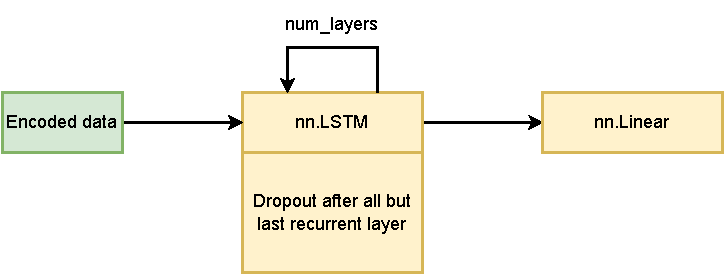
\includegraphics[width=0.7\linewidth]{lstm-arch}
    \caption{LSTM architecture.}
    \label{fig:lstm-arch}
\end{figure}

\paragraph{GRU / BiGRU} This \gls{GRU} model is identical to the \gls{LSTM}'s, only changing from the \textit{nn.LSTM} layer to \textit{nn.GRU} one. This way it is possible to directly compare these two types of recurrent neural networks.

\begin{figure}[htbp]
    \centering
    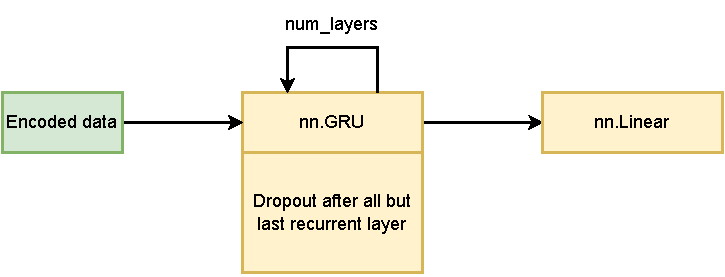
\includegraphics[width=0.7\linewidth]{gru-arch}
    \caption{GRU architecture.}
    \label{fig:gru-arch}
\end{figure}

\paragraph{CNN-LSTM / CNN-BiLSTM}

This model is a combination of the \gls{CNN} and \gls{LSTM} models. When using the \gls{CNN} model, the output of the \gls{CNN} is fed into the \gls{LSTM} model. The same previously mentioned properties of \gls{LSTM} are also present (using $num\_layers$ to create a stacked \gls{LSTM} and using $dropout$ to introduce dropout layers on the outputs of each \gls{LSTM} layers except the last one).

\begin{figure}[htbp]
    \centering
    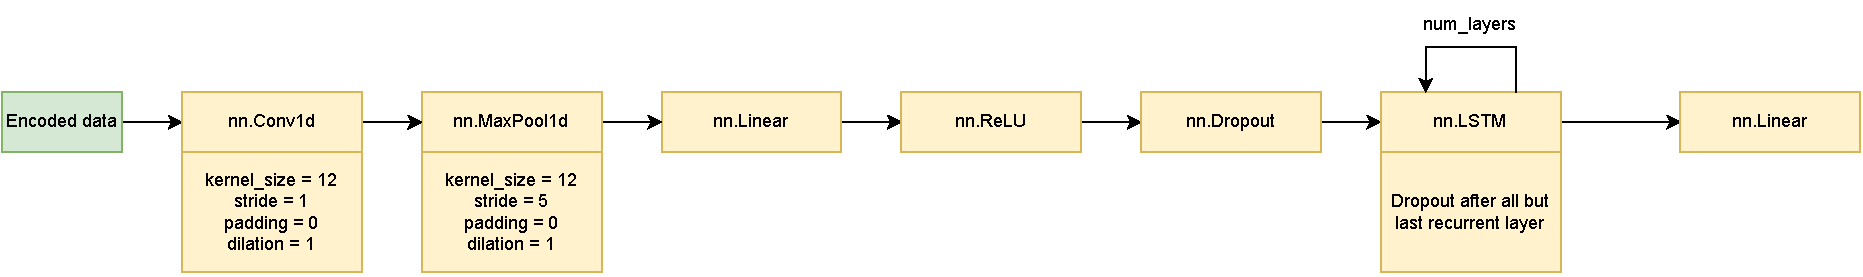
\includegraphics[width=\linewidth]{cnn-lstm-arch}
    \caption{CNN-LSTM architecture.}
    \label{fig:cnn-lstm-arch}
\end{figure}

\paragraph{CNN-GRU / CNN-BiGRU}

This model is a combination of the \gls{CNN} and \gls{GRU} models. When using the \gls{CNN} model, the output of the \gls{CNN} is fed into the \gls{GRU} model. The same previously mentioned properties of \gls{GRU} are also present (using $num\_layers$ to create a stacked \gls{GRU} and using $dropout$ to introduce dropout layers on the outputs of each \gls{GRU} layers except the last one).

\begin{figure}[htbp]
    \centering
    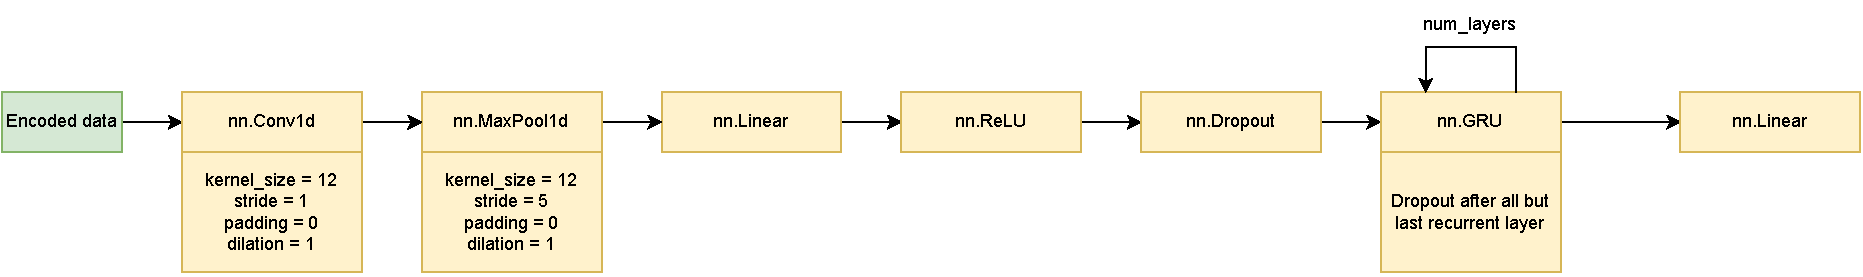
\includegraphics[width=\linewidth]{cnn-gru-arch}
    \caption{CNN-GRU architecture.}
    \label{fig:cnn-gru-arch}
\end{figure}

\subsection{Hyperparameter Tuning}

Additionally, hyperparameter optimization was considered and applied successfully. As mentioned in~\ref{sec:workflow}, the challenge of hyperparameter optimization is selecting the appropriate hyperparameters for a learning algorithm. It may distinguish an ordinary model from a very accurate one. Choosing a different learning rate or modifying the size of a network layer may have a substantial effect on the performance of the model. Ray Tune~\cite{Liaw2018Tune:Training} is the standard tuning tool for hyperparameters and it was used to complete this task. However, before finding the best combination, it is required to define the configuration of the Ray Tune's search space. The implemented one can be found in Table~\ref{tab:search_space}.

\begin{table}[ht]
	\caption{Ray Tune's search space.}
	\label{tab:search_space}
    \centering
    \begin{tabular}{lll}
    	\toprule
    	\textbf{Hyperparameter (x)} & \textbf{Search Space} \\\midrule
    	
    	Hidden Size & $x \in 32, 64, 128, 256$ \\\midrule
        Batch Size & $x \in 8, 16, 32, 64$ \\\midrule
        Learning Rate & $x \in 0.0001, 0.001, 0.01$ \\\midrule
        Dropout & $x \in 0.2, 0.3, 0.4, 0.5$ \\\midrule
        Number of Layers & $x \in 1, 2, 3$ \\
        
    	\bottomrule
    \end{tabular}
\end{table}

Ray Tune will now randomly choose a combination of parameters from these search areas for each trial. It will then train many models in parallel and determine which one has the highest performance. Additionally, the Ray Tune's scheduler \textit{ASHAScheduler} was used, which terminates poorly performing trials early. This is accomplished by choosing a desired metric (loss in this study) and measuring it at the end of each epoch. If the measure keeps worsening, reaching a specified patience value, the trial will end immediately. 

\subsection{Other Parameters}

The process of early stopping is a very useful technique since it prevents wasting time and resources on unnecessary computations. Therefore, this strategy was also implemented in the case when hyperparameter tuning is not being performed, using now the \textit{ReduceLROnPlateau} scheduler from \textit{PyTorch}. This scheduler is also able to reduce the learning rate when the given metric has stopped improving, since models often benefit from a 2-10x reduction in the learning rate when learning has stagnated.